\documentclass{beamer}

\usepackage[utf8]{inputenc}
\usepackage[ngerman]{babel}
\usepackage[T1]{fontenc}
\usepackage{graphicx}
\usepackage{amssymb}
\usepackage{pifont}
\usepackage{tikz}
\usepackage{tikzsymbols}
\usepackage{booktabs}
\usepackage{minted}

\newcommand{\cmark}{\ding{51}}
\newcommand{\xmark}{\ding{55}}

\usetheme{Singapore}

\graphicspath{{./images/}{./images/logos/}}

\setbeamertemplate{itemize subitem}{$\blacktriangleright$}
%\renewcommand{\labelitemii}{$\blacktriangleright$}

\begin{document}

\title{Softwareentwicklungsprozess: \\ Vorschl"age}
\date{\today}
\author{Oleg H"ofling}
\institute[netqa]{netqa GmbH}
\logo{
	\includegraphics[scale=.05]{netqa-logo.eps}
} % end logo
\frame{\maketitle}

\frame{\frametitle{"Uberblick}\tableofcontents[hideallsubsections]}

\section{Ziele}
\subsection{Placeholder}
\begin{frame}
	\begin{itemize}
		\item[\cmark] Eigene Vorschl"age "ubermitteln
		\item[\cmark] \textbf{Konstruktive} Kritik (eher wenig)
		\item[\cmark] Aufgaben in akute und langfristige aufteilen
		\item[\cmark] Anregung zur Diskussion
	\end{itemize}
\end{frame}

\section{Joel Test}
\subsection{Placeholder}
\begin{frame}{Joel Spolsky}
	\begin{columns}[T] % align columns
		\begin{column}{.49\textwidth}
			\vfill
			\begin{center}
				\includegraphics[scale=.25]{spolsky.jpeg}
			\end{center}
			\vfill
		\end{column}
		\hfill
		\begin{column}[t]{0.49\textwidth}
			\vfill
				\includegraphics[scale=.25]{so-logo.eps}
			\vfill
				
\includegraphics[scale=.25]{trello-logo-blue.eps}
			\vfill
				
\includegraphics[scale=.75]{fogbugz.eps}
		\end{column}
	\end{columns}
\end{frame}

\begin{frame}{Der Joel Test}
	\begin{itemize}
		\item Einfach und schnell
		\item Es wird der \textbf{Softwareentwicklungsprozess} evaluiert
		\item 12 Fragen, ein Punkt f"ur jede \glqq{}Ja\grqq{}-Antwort
		\item Auswertung:
			\begin{description}[labelwidth=\widthof{10 Punkte:}]
				\item[12 Punkte:] \Laughey
				\item[11 Punkte:] \Neutrey
				\item[$\leqslant 10$ Punkte:] \Xey
			\end{description}
	\end{itemize}
\end{frame}

\begin{frame}{Der Joel Test, Teil I}
	\begin{enumerate}
		\item<1-> Do you use source control? \uncover<2->{\cmark}
		\item<3-> Can you make a build in one step? \uncover<4->{\xmark}
		\item<5-> Do you make daily builds? \uncover<6->{\xmark}
		\item<7-> Do you have a bug database? \uncover<8->{\cmark}
		\item<9-> Do you fix bugs before writing new code? \uncover<10->{\cmark}
		\item<11-> Do you have an up-to-date schedule? \uncover<12->{\xmark}
	\end{enumerate}
\end{frame}

\begin{frame}{Der Joel Test, Teil II}
	\begin{enumerate}
		\setcounter{enumi}{6}
		\item<1-> Do you have a spec? \uncover<2->{\xmark}
		\item<3-> Do programmers have quiet working conditions? \uncover<4->{\cmark}
		\item<5-> Do you use the best tools money can buy? \uncover<6->{\cmark}
		\item<7-> Do you have testers? \uncover<8->{\cmark}
		\item<9-> Do new candidates write code during their interview? \uncover<10->{\xmark}
		\item<11-> Do you do hallway usability testing? \uncover<12->{\xmark}
	\end{enumerate}
\end{frame}

\begin{frame}{Ergebnis}
	\begin{center}
		\includegraphics[scale=.25]{sad-kid.jpg}
	\end{center}
\end{frame}

\section{Operative Ziele}
\subsection{Placeholder}
\begin{frame}{Git Flow}
	\begin{columns}[T] % align columns
		\begin{column}{.2\textwidth}
			\resizebox{!}{.8\textheight}{
					\begin{tikzpicture}
\tikzstyle{commit}=[draw,circle,fill=white,inner sep=0pt,minimum size=5pt]
\tikzstyle{clabel}=[right,outer sep=1em]
\tikzstyle{every path}=[draw]
\tikzstyle{branch}=[draw,rect,fill=yellow,inner sep=0pt,minimum size=5pt]

\node[commit] (fa6af28) at (0.0,-273.5) {};
\node[right,xshift=5.5] (label_fa6af28) at (fa6af28.east) {\verb!fa6af28!};
\node[commit] (13d3ed7) at (0.0,-274.0) {};
\node[right,xshift=6.0] (label_13d3ed7) at (13d3ed7.east) {\verb!13d3ed7!};
\draw[->] (13d3ed7) -- (fa6af28);
\node[commit] (6789c7d) at (0.0,-274.5) {};
\node[right,xshift=6.0] (label_6789c7d) at (6789c7d.east) {\verb!6789c7d!};
\draw[->] (6789c7d) -- (13d3ed7);
\node[commit] (ed6a90e) at (0.5,-275.0) {};
\node[right,xshift=7.0] (label_ed6a90e) at (ed6a90e.east) {\verb!ed6a90e!};
\draw[->] (ed6a90e) -- (6789c7d);
\node[commit] (1560e00) at (1.0,-275.5) {};
\node[right,xshift=5.5] (label_1560e00) at (1560e00.east) {\verb!1560e00!};
\draw[->] (1560e00) -- (ed6a90e);
\node[commit] (91fde5b) at (0.5,-276.0) {};
\node[right,xshift=5.5] (label_91fde5b) at (91fde5b.east) {\verb!91fde5b!};
\draw[->] (91fde5b) -- (ed6a90e);
\node[commit] (9258f19) at (0.0,-276.5) {};
\node[right,xshift=6.0] (label_9258f19) at (9258f19.east) {\verb!9258f19!};
\draw[->] (9258f19) -- (6789c7d);
\draw[->] (9258f19) -- (91fde5b);
\node[commit] (d4f9e15) at (0.5,-277.0) {};
\node[right,xshift=7.0] (label_d4f9e15) at (d4f9e15.east) {\verb!d4f9e15!};
\draw[->] (d4f9e15) -- (1560e00);
\draw[->] (d4f9e15) -- (9258f19);
\node[commit] (4f39c11) at (1.0,-277.5) {};
\node[right,xshift=6.5] (label_4f39c11) at (4f39c11.east) {\verb!4f39c11!};
\draw[->] (4f39c11) -- (d4f9e15);
\node[commit] (b906233) at (0.5,-278.0) {};
\node[right,xshift=6.0] (label_b906233) at (b906233.east) {\verb!b906233!};
\draw[->] (b906233) -- (d4f9e15);
\node[commit] (bd8c693) at (0.0,-278.5) {};
\node[right,xshift=9.5] (label_bd8c693) at (bd8c693.east) {\verb!bd8c693!};
\draw[->] (bd8c693) -- (9258f19);
\draw[->] (bd8c693) -- (b906233);
\node[commit] (ea4f705) at (0.0,-279.0) {};
\node[right,xshift=6.5] (label_ea4f705) at (ea4f705.east) {\verb!ea4f705!};
\draw[->] (ea4f705) -- (bd8c693);
\node[commit] (8a96668) at (0.0,-279.5) {};
\node[right,xshift=3.0] (label_8a96668) at (8a96668.east) {\verb!8a96668!};
\draw[->] (8a96668) -- (4f39c11);
\draw[->] (8a96668) -- (ea4f705);
\node[commit] (304b154) at (0.0,-280.0) {};
\node[right,xshift=5.0] (label_304b154) at (304b154.east) {\verb!304b154!};
\draw[->] (304b154) -- (8a96668);
\node[commit] (972bb24) at (0.5,-280.5) {};
\node[right,xshift=3.0] (label_972bb24) at (972bb24.east) {\verb!972bb24!};
\draw[->] (972bb24) -- (304b154);
\node[commit] (aada0eb) at (0.5,-281.0) {};
\node[right,xshift=6.5] (label_aada0eb) at (aada0eb.east) {\verb!aada0eb!};
\draw[->] (aada0eb) -- (972bb24);
\node[commit] (59a8934) at (1.0,-281.5) {};
\node[right,xshift=3.5] (label_59a8934) at (59a8934.east) {\verb!59a8934!};
\draw[->] (59a8934) -- (aada0eb);
\node[commit] (6787b2f) at (1.0,-282.0) {};
\node[right,xshift=6.0] (label_6787b2f) at (6787b2f.east) {\verb!6787b2f!};
\draw[->] (6787b2f) -- (59a8934);
\node[commit] (610309a) at (1.0,-282.5) {};
\node[right,xshift=8.5] (label_610309a) at (610309a.east) {\verb!610309a!};
\draw[->] (610309a) -- (6787b2f);
\node[commit] (8fc8404) at (1.0,-283.0) {};
\node[right,xshift=5.0] (label_8fc8404) at (8fc8404.east) {\verb!8fc8404!};
\draw[->] (8fc8404) -- (610309a);
\node[commit] (d1743ee) at (1.0,-283.5) {};
\node[right,xshift=5.5] (label_d1743ee) at (d1743ee.east) {\verb!d1743ee!};
\draw[->] (d1743ee) -- (8fc8404);
\node[commit] (e5f1da5) at (1.0,-284.0) {};
\node[right,xshift=7.0] (label_e5f1da5) at (e5f1da5.east) {\verb!e5f1da5!};
\draw[->] (e5f1da5) -- (d1743ee);
\node[commit] (13c2800) at (1.0,-284.5) {};
\node[right,xshift=8.0] (label_13c2800) at (13c2800.east) {\verb!13c2800!};
\draw[->] (13c2800) -- (e5f1da5);
\node[commit] (614b139) at (1.5,-285.0) {};
\node[right,xshift=4.5] (label_614b139) at (614b139.east) {\verb!614b139!};
\draw[->] (614b139) -- (13c2800);
\node[commit] (385ece3) at (1.5,-285.5) {};
\node[right,xshift=6.0] (label_385ece3) at (385ece3.east) {\verb!385ece3!};
\draw[->] (385ece3) -- (614b139);
\node[commit] (9961ea4) at (1.5,-286.0) {};
\node[right,xshift=6.0] (label_9961ea4) at (9961ea4.east) {\verb!9961ea4!};
\draw[->] (9961ea4) -- (385ece3);
\node[commit] (8661295) at (1.5,-286.5) {};
\node[right,xshift=8.0] (label_8661295) at (8661295.east) {\verb!8661295!};
\draw[->] (8661295) -- (9961ea4);
\node[commit] (25a17c6) at (0.0,-287.0) {};
\node[right,xshift=6.5] (label_25a17c6) at (25a17c6.east) {\verb!25a17c6!};
\draw[->] (25a17c6) -- (304b154);
\node[commit] (fe93cbf) at (0.5,-287.5) {};
\node[right,xshift=4.0] (label_fe93cbf) at (fe93cbf.east) {\verb!fe93cbf!};
\draw[->] (fe93cbf) -- (aada0eb);
\draw[->] (fe93cbf) -- (25a17c6);
\node[commit] (2afbe7d) at (0.5,-288.0) {};
\node[right,xshift=6.5] (label_2afbe7d) at (2afbe7d.east) {\verb!2afbe7d!};
\draw[->] (2afbe7d) -- (fe93cbf);
\node[commit] (4f8c57f) at (0.5,-288.5) {};
\node[right,xshift=9.0] (label_4f8c57f) at (4f8c57f.east) {\verb!4f8c57f!};
\draw[->] (4f8c57f) -- (2afbe7d);
\node[commit] (9438db5) at (0.5,-289.0) {};
\node[right,xshift=5.5] (label_9438db5) at (9438db5.east) {\verb!9438db5!};
\draw[->] (9438db5) -- (4f8c57f);
\node[commit] (f57ad96) at (0.5,-289.5) {};
\node[right,xshift=6.0] (label_f57ad96) at (f57ad96.east) {\verb!f57ad96!};
\draw[->] (f57ad96) -- (9438db5);
\node[commit] (95c0b3c) at (0.5,-290.0) {};
\node[right,xshift=7.5] (label_95c0b3c) at (95c0b3c.east) {\verb!95c0b3c!};
\draw[->] (95c0b3c) -- (f57ad96);
\node[commit] (ff4d68f) at (0.5,-290.5) {};
\node[right,xshift=6.0] (label_ff4d68f) at (ff4d68f.east) {\verb!ff4d68f!};
\draw[->] (ff4d68f) -- (95c0b3c);
\node[commit] (f9e73b7) at (0.0,-291.0) {};
\node[right,xshift=5.5] (label_f9e73b7) at (f9e73b7.east) {\verb!f9e73b7!};
\draw[->] (f9e73b7) -- (25a17c6);
\draw[->] (f9e73b7) -- (ff4d68f);
\node[commit] (eac19e6) at (0.0,-291.5) {};
\node[right,xshift=6.0] (label_eac19e6) at (eac19e6.east) {\verb!eac19e6!};
\draw[->] (eac19e6) -- (f9e73b7);
\node[commit] (a1d0a3d) at (0.5,-292.0) {};
\node[right,xshift=4.0] (label_a1d0a3d) at (a1d0a3d.east) {\verb!a1d0a3d!};
\draw[->] (a1d0a3d) -- (13c2800);
\draw[->] (a1d0a3d) -- (eac19e6);
\node[commit] (677c451) at (0.5,-292.5) {};
\node[right,xshift=5.5] (label_677c451) at (677c451.east) {\verb!677c451!};
\draw[->] (677c451) -- (a1d0a3d);
\node[commit] (61609d7) at (0.5,-293.0) {};
\node[right,xshift=5.5] (label_61609d7) at (61609d7.east) {\verb!61609d7!};
\draw[->] (61609d7) -- (677c451);
\node[commit] (56c761b) at (0.5,-293.5) {};
\node[right,xshift=7.5] (label_56c761b) at (56c761b.east) {\verb!56c761b!};
\draw[->] (56c761b) -- (61609d7);
\node[commit] (ba794a9) at (0.0,-294.0) {};
\node[right,xshift=6.5] (label_ba794a9) at (ba794a9.east) {\verb!ba794a9!};
\draw[->] (ba794a9) -- (eac19e6);
\draw[->] (ba794a9) -- (56c761b);
\node[commit] (c7b6569) at (0.0,-294.5) {};
\node[right,xshift=3.5] (label_c7b6569) at (c7b6569.east) {\verb!c7b6569!};
\draw[->] (c7b6569) -- (8661295);
\draw[->] (c7b6569) -- (ba794a9);
\node[commit] (05d7327) at (0.0,-295.0) {};
\node[right,xshift=5.0] (label_05d7327) at (05d7327.east) {\verb!05d7327!};
\draw[->] (05d7327) -- (c7b6569);

\end{tikzpicture}

			}
		\end{column}
		\hfill
		\begin{column}{.8\textwidth}
			\vfill
			\begin{itemize}
				\item<1-> So sieht's im Moment aus
				\item<1-> Keine Struktur zu erkennen
				\item<1-> Futter f"ur Mergekonflikte
				\item<1-> Fehlersuche mit \texttt{git bisect} wird erschwert
				\item<2->[] \fbox{\includegraphics[scale=.33]{git-rebase-coming.jpg}}
			\end{itemize}
		\end{column}
	\end{columns}
\end{frame}

\begin{frame}{Git Flow}
	\begin{center}
		\resizebox{!}{.8\textheight}{
			\begin{tikzpicture}

\tikzstyle{commit}=[draw,circle,fill=white,inner sep=0pt,minimum size=5pt]
\tikzstyle{clabel}=[right,outer sep=1em]
\tikzstyle{every path}=[draw]
\tikzstyle{branch}=[draw,rectangle,fill=yellow,inner sep=.5ex,minimum width=2ex, minimum height=2ex]
\tikzstyle{tag}=[draw,rectangle,fill=blue!30,inner sep=.5ex,minimum width=2ex, minimum height=2ex]

\node[commit] (966a68d) at (0.0,0) {};
\node[right,xshift=4.0] (label_966a68d) at (966a68d.east) {\verb!966a68d Merge branch 'another-cool-feature' into develop!};
\node[commit] (7f8a836) at (0.5,-0.5) {};
\node[right,xshift=4.0] (label_7f8a836) at (7f8a836.east) {\verb!7f8a836 [another-cool-feature] added tests for feature!};
\draw[->] (7f8a836) -- (966a68d);
\node[commit] (d4dbe5f) at (0.5,-1.0) {};
\node[right,xshift=3.5] (label_d4dbe5f) at (d4dbe5f.east) {\verb!d4dbe5f [another-cool-feature] finished feature impl!};
\draw[->] (d4dbe5f) -- (7f8a836);
\node[commit] (f7b18ac) at (0.5,-1.5) {};
\node[right,xshift=5.5] (label_f7b18ac) at (f7b18ac.east) {\verb!f7b18ac [another-cool-feature] work on another cool feature in progress!};
\draw[->] (f7b18ac) -- (d4dbe5f);
\node[commit] (eb0d9c6) at (0.5,-2.0) {};
\node[right,xshift=5.0] (label_eb0d9c6) at (eb0d9c6.east) {\verb!eb0d9c6 [another-cool-feature] started work on another cool feature!};
\draw[->] (eb0d9c6) -- (f7b18ac);
\node[commit] (c95ac20) at (-0.5,-2.5) {};
\node[right,xshift=22.5] (label_c95ac20) at (c95ac20.east) {\verb!c95ac20 Merge branch 'develop' into master!};
\node[commit] (4f16a13) at (0.0,-3.0) {};
\node[right,xshift=4.5] (label_4f16a13) at (4f16a13.east) {\verb!4f16a13 Merge branch 'some-new-feature' into develop!};
\draw[->] (4f16a13) -- (966a68d);
\draw[->] (4f16a13) -- (eb0d9c6);
\draw[->] (4f16a13) -- (c95ac20);
\node[commit] (3e38c7f) at (0.5,-3.5) {};
\node[right,xshift=4.0] (label_3e38c7f) at (3e38c7f.east) {\verb!3e38c7f [some-new-feature] added feature tests!};
\draw[->] (3e38c7f) -- (4f16a13);
\node[commit] (c4e82e1) at (0.5,-4.0) {};
\node[right,xshift=4.0] (label_c4e82e1) at (c4e82e1.east) {\verb!c4e82e1 [some-new-feature] continuing feature impl!};
\draw[->] (c4e82e1) -- (3e38c7f);
\node[commit] (46e4577) at (0.5,-4.5) {};
\node[right,xshift=6.5] (label_46e4577) at (46e4577.east) {\verb!46e4577 [some-new-feature] found and fixed a bug in feature code!};
\draw[->] (46e4577) -- (c4e82e1);
\node[commit] (82857ce) at (0.5,-5.0) {};
\node[right,xshift=5.5] (label_82857ce) at (82857ce.east) {\verb!82857ce [some-new-feature] started working on a new feature!};
\draw[->] (82857ce) -- (46e4577);
\node[commit] (9271ce9) at (-0.5,-5.5) {};
\node[right,xshift=22.5] (label_9271ce9) at (9271ce9.east) {\verb!9271ce9 Merge branch 'develop' into master!};
\draw[->] (9271ce9) -- (c95ac20);
\node[commit] (5934940) at (0.0,-6.0) {};
\node[right,xshift=4.5] (label_5934940) at (5934940.east) {\verb!5934940 Merge branch 'feature3' into develop!};
\draw[->] (5934940) -- (4f16a13);
\draw[->] (5934940) -- (82857ce);
\draw[->] (5934940) -- (9271ce9);
\node[commit] (239c589) at (0.5,-6.5) {};
\node[right,xshift=4.0] (label_239c589) at (239c589.east) {\verb!239c589 [feature3] added gui tests!};
\draw[->] (239c589) -- (5934940);
\node[commit] (4d0c539) at (0.5,-7.0) {};
\node[right,xshift=5.0] (label_4d0c539) at (4d0c539.east) {\verb!4d0c539 [feature3] finalized gui updates via controller!};
\draw[->] (4d0c539) -- (239c589);
\node[commit] (677b82c) at (0.5,-7.5) {};
\node[right,xshift=7.0] (label_677b82c) at (677b82c.east) {\verb!677b82c [feature3] added gui classes, first try of controller updating guis!};
\draw[->] (677b82c) -- (4d0c539);
\node[commit] (4d28070) at (0.0,-8.0) {};
\node[right,xshift=4.5] (label_4d28070) at (4d28070.east) {\verb!4d28070 Merge branch 'feature2' into develop!};
\draw[->] (4d28070) -- (5934940);
\draw[->] (4d28070) -- (677b82c);
\node[commit] (59e331d) at (0.5,-8.5) {};
\node[right,xshift=7.0] (label_59e331d) at (59e331d.east) {\verb!59e331d [feature2] implemented controller functions, added tests with data model mocks!};
\draw[->] (59e331d) -- (4d28070);
\node[commit] (53d43d8) at (0.5,-9.0) {};
\node[right,xshift=4.0] (label_53d43d8) at (53d43d8.east) {\verb!53d43d8 [feature2] added controller skeleton!};
\draw[->] (53d43d8) -- (59e331d);
\node[commit] (abf4c95) at (0.0,-9.5) {};
\node[right,xshift=4.5] (label_abf4c95) at (abf4c95.east) {\verb!abf4c95 Merge branch 'feature1' into develop!};
\draw[->] (abf4c95) -- (4d28070);
\draw[->] (abf4c95) -- (53d43d8);
\node[commit] (e2b7b2b) at (0.5,-10.0) {};
\node[right,xshift=4.0] (label_e2b7b2b) at (e2b7b2b.east) {\verb!e2b7b2b [feature1] wrote serializer tests!};
\draw[->] (e2b7b2b) -- (abf4c95);
\node[commit] (082e597) at (0.5,-10.5) {};
\node[right,xshift=5.0] (label_082e597) at (082e597.east) {\verb!082e597 [feature1] added serializers for data classes!};
\draw[->] (082e597) -- (e2b7b2b);
\node[commit] (b9873f8) at (0.5,-11.0) {};
\node[right,xshift=4.5] (label_b9873f8) at (b9873f8.east) {\verb!b9873f8 [feature1] implemented data model classes!};
\draw[->] (b9873f8) -- (082e597);
\node[commit] (55dc85f) at (0.5,-11.5) {};
\node[right,xshift=4.5] (label_55dc85f) at (55dc85f.east) {\verb!55dc85f [feature1] working on feature started!};
\draw[->] (55dc85f) -- (b9873f8);
\node[commit] (eb85dd5) at (0.0,-12.0) {};
\node[right,xshift=3.5] (label_eb85dd5) at (eb85dd5.east) {\verb!eb85dd5 started branch for developing!};
\draw[->] (eb85dd5) -- (abf4c95);
\draw[->] (eb85dd5) -- (55dc85f);
\node[commit] (dcbd56b) at (-0.5,-12.5) {};
\node[right,xshift=1.5] (label_dcbd56b) at (dcbd56b.east) {\verb!dcbd56b initialised repo!};
\draw[->] (dcbd56b) -- (9271ce9);
\draw[->] (dcbd56b) -- (eb85dd5);
\node[branch,right,xshift=.1] (develop) at (label_966a68d.east) {\verb!develop!};
\node[branch,right,xshift=.1] (master) at (label_c95ac20.east) {\verb!master!};
\node[tag,right,xshift=.1] (label_tag_v1.0) at (label_9271ce9.east) {\verb!v1.0!};
\node[tag,right,xshift=1.1] (label_tag_v2.0) at (master.east) {\verb!v2.0!};
\end{tikzpicture}

		}
	\end{center}
\end{frame}

\begin{frame}{Git Flow}
	\begin{center}
		Man kann es weiter ausbauen$\ldots$
		
		\includegraphics[height=.8\textheight]{git-model.png}
	\end{center}
\end{frame}

\begin{frame}{Git Flow}
	\begin{itemize}
		\item Prozess in Trello (vollst"andig?) dokumentiert
		\item Kleine Commits (duh!)
		\item Sinnvolle Branchnamen und Commit Messages
		\item[] Insbesondere \texttt{indev\char`_py3} umbenennen
		\item Branchname als Prefix im Commit Message
	\end{itemize}
\end{frame}

\begin{frame}{Git Flow}
	\only<1>{
		\resizebox{!}{.6\textheight}{
			\begin{tikzpicture}
\tikzstyle{commit}=[draw,circle,fill=white,inner sep=0pt,minimum size=5pt]
\tikzstyle{every path}=[draw]

\node[commit] (b2278ea) at (0.0,-15.0) {};
\node[right,xshift=10] (label_b2278ea) at (b2278ea.east) {\verb!b2278ea: added project ref in run!};
\node[commit] (65d08e1) at (0.0,-15.5) {};
\node[right,xshift=10] (label_65d08e1) at (65d08e1.east) {\verb!65d08e1: added netqa logo & home page link!};
\path (65d08e1) to[out=90,in=-90] (b2278ea);
\node[commit] (0e1b221) at (0.0,-16.0) {};
\node[right,xshift=10] (label_0e1b221) at (0e1b221.east) {\verb!0e1b221: added simple data model for test runs!};
\path (0e1b221) to[out=90,in=-90] (65d08e1);
\node[commit] (aa2b001) at (0.0,-16.5) {};
\node[right,xshift=10] (label_aa2b001) at (aa2b001.east) {\verb!aa2b001: Merge branch 'django-channels' into django-sandbox!};
\path (aa2b001) to[out=90,in=-90] (0e1b221);
\node[commit] (fbdac0d) at (0.5,-17.0) {};
\node[right,xshift=10] (label_fbdac0d) at (fbdac0d.east) {\verb!fbdac0d: added control elements for docs and help!};
\path (fbdac0d) to[out=90,in=-90] (aa2b001);
\node[commit] (421e99e) at (0.5,-17.5) {};
\node[right,xshift=10] (label_421e99e) at (421e99e.east) {\verb!421e99e: renamed client events!};
\path (421e99e) to[out=90,in=-90] (fbdac0d);
\node[commit] (e1b5521) at (0.5,-18.0) {};
\node[right,xshift=10] (label_e1b5521) at (e1b5521.east) {\verb!e1b5521: fixed module deps!};
\path (e1b5521) to[out=90,in=-90] (421e99e);
\node[commit] (f1ccf26) at (0.5,-18.5) {};
\node[right,xshift=10] (label_f1ccf26) at (f1ccf26.east) {\verb!f1ccf26: created client-independent utils package!};
\path (f1ccf26) to[out=90,in=-90] (e1b5521);
\node[commit] (42a8ebb) at (0.5,-19.0) {};
\node[right,xshift=10] (label_42a8ebb) at (42a8ebb.east) {\verb!42a8ebb: first impl of websocket client endpoint!};
\path (42a8ebb) to[out=90,in=-90] (f1ccf26);
\node[commit] (b404edb) at (0.5,-19.5) {};
\node[right,xshift=10] (label_b404edb) at (b404edb.east) {\verb!b404edb: added angular websocket dependency!};
\path (b404edb) to[out=90,in=-90] (42a8ebb);
\node[commit] (4b7bbf9) at (0.5,-20.0) {};
\node[right,xshift=10] (label_4b7bbf9) at (4b7bbf9.east) {\verb!4b7bbf9: introduced url builder, particularly for ws url conversion!};
\path (4b7bbf9) to[out=90,in=-90] (b404edb);
\node[commit] (84c0039) at (0.5,-20.5) {};
\node[right,xshift=10] (label_84c0039) at (84c0039.east) {\verb!84c0039: some simple event handling added!};
\path (84c0039) to[out=90,in=-90] (4b7bbf9);
\node[commit] (134b5ad) at (0.5,-21.0) {};
\node[right,xshift=10] (label_134b5ad) at (134b5ad.east) {\verb!134b5ad: added websocket!};
\path (134b5ad) to[out=90,in=-90] (84c0039);
\node[commit] (6ba0de8) at (0.0,-21.5) {};
\node[right,xshift=10] (label_6ba0de8) at (6ba0de8.east) {\verb!6ba0de8: explicitly adding static url patterns to url config!};
\path (6ba0de8) to[out=90,in=-90] (aa2b001);
\path (6ba0de8) to[out=90,in=-90] (134b5ad);
\node[commit] (f5dfbfc) at (0.0,-22.0) {};
\node[right,xshift=10] (label_f5dfbfc) at (f5dfbfc.east) {\verb!f5dfbfc: boilerplate code for the project scan!};
\path (f5dfbfc) to[out=90,in=-90] (6ba0de8);
\end{tikzpicture}
		}
	}
	\only<2>{
		\resizebox{!}{.6\textheight}{
			\input{git-branch-names}
		}
	}
\end{frame}

\begin{frame}{Git Flow}
	\begin{columns}[T] % align columns
		\begin{column}{.4\textwidth}
			\begin{center}
				\includegraphics[scale=.2]{progit.png}
			\end{center}
		\end{column}
		\hfill
		\begin{column}{.8\textwidth}
			\vfill
			\begin{itemize}
				\item \texttt{Git Command Line} verwenden
				\item Terminal einrichten
					\begin{itemize}
						\item Tab-Vervollst"andigung
						\item Vorw"arts-/R"uckw"artssuche im Command Log
						\item Farben
					\end{itemize}
				\item Repo Browser verwenden
					\begin{description}[Windows]
						\item[Windows] GitExtensions, SourceTree
						\item[Linux] gitg, git-cola
					\end{description}
				\item Handbuch: Pro Git, 2nd Edition (kostenlos!)
			\end{itemize}
		\end{column}
	\end{columns}
\end{frame}

\begin{frame}{Statische Codeanalyse}
	\begin{itemize}
		\item Einheitliche Formatierung
			\begin{itemize}
				\item Ein Tab ist 4 Leerzeichen lang
				\item Klassen: \texttt{CamelCase}
				\item Variablen: \texttt{lower\char`_case\char`_with\char`_underscores}
				\item Keine Leerzeichen am Zeilenende
				\item \texttt{text = 'netqa'} oder \texttt{text = "netqa"}?
			\end{itemize}
		\item Potenzielle Bugs fr"uh abfangen
		\item Unn"otige Merge-Konflikte vermeiden
		\item Disziplin
	\end{itemize}
\end{frame}

\begin{frame}{Statische Codeanalyse: Python}
	\begin{itemize}
		\item Minimalsatz an Regeln ausarbeiten		
		\item \texttt{PEP\,8} und \texttt{Pylint}
		\item Automatisches Stylechecking vor dem Commit bereits eingerichtet (\texttt{origin/git-repo-setup})
		\item Aktuell 1554 Verletzungen
		\item \texttt{Pylint} bietet Code-Rating an:
	\end{itemize}
	\begin{center}
		\begin{minipage}{.8\textwidth}
			\texttt{Global evaluation}

			\texttt{-----------------}

			\texttt{Your code has been rated at 6.02/10 (previous run: 6.46/10, -0.44)}
		\end{minipage}
	\end{center}
\end{frame}

\begin{frame}{Statische Codeanalyse: Javascript}
	\begin{itemize}
		\item Anwendung:
			\begin{itemize}
				\item Dashboard \cmark
				\item Reports?
			\end{itemize}
		\item Kein etablierter Linter
		\item Strict-Mode f"ur JS-Compilers:
		\item[] \texttt{'use strict';}
	\end{itemize}
\end{frame}

\begin{frame}{Code Review}
	\begin{itemize}
		\item In einer idealen Welt: immer
		\item Vier-Augen-Prinzip
		\item Kann z.\,B. durch Scrum erzwungen werden
	\end{itemize}
\end{frame}

\begin{frame}{Nightly Builds}
	\begin{itemize}
		\item Build = Endprodukt
		\item Der Build-Prozess fehlt!
		\item Standalone Installer?
		\item Web Service Deployment?
		\item $\ldots$?
	\end{itemize}
\end{frame}

\begin{frame}{Nightly Builds}
	Minimale Integration in Jenkins:
	\begin{itemize}
		\item Cron-Job, startet um 23 Uhr
		\item Baut \texttt{develop} und \texttt{release/master}
		\item Setzt Tags in \texttt{Git} (Version usw)
		\item F"uhrt Unit Tests aus
		\item F"uhrt Systemtests aus
		\item Report wird am n"achsten Morgen evaluiert
		\item Standalone: Stabile Builds werden Kunden zum Download angeboten
		\item Web Service: Deployment auf den Production Server
		\item Build"ubergreifende Metriken auswerten
	\end{itemize}
\end{frame}

\begin{frame}[fragile]{Tests}
	\begin{itemize}
		\item Aktuell: 62\% Abdeckung
		\item Gar nicht mal so "ubel, wenn \texttt{coverage} richtig liegt
		\item Systemtests (wenn der Build-Prozess steht)
	\end{itemize}
	
	\begin{overprint}
	\onslide<1>
	\begin{minted}{bash}
	$ nosetests --with-coverage \
		--cover-package=NetqaFwRoot
	---------------------------
	Name   Stmts   Miss   Cover
	TOTAL  1545    592    62%
	---------------------------
	Ran 53 tests in 20.421s
	FAILED (SKIP=1, errors=8)
	\end{minted}
	
	\onslide<2>
	\begin{minted}{bash}
	$ find NetqaFwRoot/ -type f -iname '*.py' \
		-not -path "*/tests/*" \
		| xargs sed '/^\s*#/d;/^\s*$/d' \
		| wc -l
	4846
	\end{minted}
	\end{overprint}
\end{frame}

\begin{frame}{Versionierung}
	\begin{equation*}
		\underbrace{\underbrace{\underbrace{1}_{\text{Major}}.\underbrace{5}_{\text{Minor}}}_{\text{Release}}.\underbrace{11}_{\text{Features}}.\underbrace{255}_{\text{Survived Days}}}_{\text{Develop}}
	\end{equation*}
	\vfill
	\begin{description}[Survived Days:]
		\item[Major:] Version vom letzten Release
		\item[Minor:] Bugfixing-Releases
		\item[Features:] Anzahl Features im aktuellen Develop
		\item[Survived Days:] Anzahl Tage seit dem letzten Release
		\item[Ansonsten:] \texttt{PEP\,396 -- Module Version Numbers}
	\end{description}
\end{frame}

\section{Strategische Ziele}
\subsection{Placeholder}

\begin{frame}{"Ubersicht}
	\begin{itemize}
		\item Specification-Dokument
			\begin{itemize}
				\item Systemanforderungen
				\item Funktionalit"at
				\item Interfaces nach au"sen
				\item Screenshots vom GUI bzw. Mockups
				\item "Anderungen werden auch versioniert
			\end{itemize}
		\item Agiler Prozess
			\begin{itemize}
				\item Zu umfangreich -- separate Pr"asi?
				\item (Au"serdem keine guten Folien vorbereitet \Sadey)
				\item Kommt erst nach dem Spec
			\end{itemize}
	\end{itemize}
\end{frame}

\begin{frame}{Agiler Prozess}
	\begin{itemize}
		\item Ziel: schnell Ergebnisse liefern
		\item Ein Entwicklungszyklus wird in 2-3 Wochen abgeschlossen (Rolling Release)
		\item Deckt ab:
			\begin{itemize}
				\item Projektplanung
				\item Zeitmanagement
				\item Bugfixing
				\item Implementation von neuen Features
			\end{itemize}
		\item $\text{Scrum} + \text{JIRA} = \Laughey$, $\text{Kanban} + \text{Trello} = \Neutrey$, $\ldots$?
	\end{itemize}
\end{frame}

\begin{frame}{Scrum-Zyklus}
	\begin{center}
		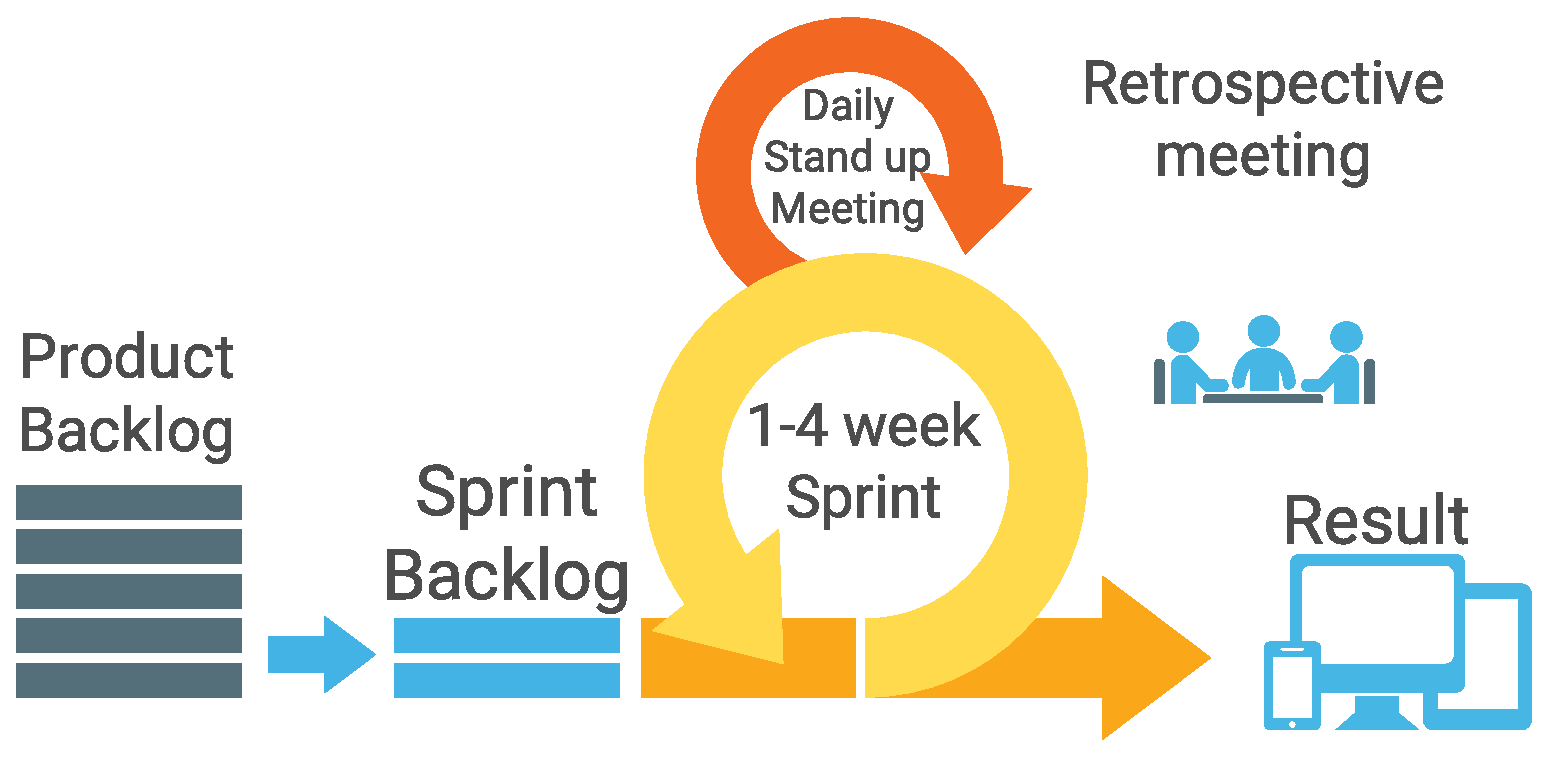
\includegraphics[scale=.25]{scrum-process.eps}
	\end{center}
\end{frame}

\begin{frame}{Ticket-Lebenszyklus}
	\begin{center}
		\includegraphics[scale=.5]{jira-ticket-lifecycle.png}
	\end{center}
\end{frame}

\begin{frame}{Scrum, Regeln}
	\begin{itemize}
		\item Alle Bugs werden im Bug Tracker persistiert
		\item M"undlich berichtete Bugs (\glqq{}Den Fehler habe ich doch schon vor Wochen gesehen$\ldots$\grqq) werden ignoriert
		\item Alle Ideen werden im Product Backlog persistiert
		\item M"undlich ge"au"serte W"unsche (\glqq{}Kannst Du noch schnell ein Button einbauen?$\ldots$\grqq) werden ignoriert
		\item B"urokratie \xmark
		\item Aber: Nach der Gew"ohnungsphase dauert das Erstellen von Tickets selten mehr als 5 Minuten
		\item Nichts geht verloren \cmark
	\end{itemize}
\end{frame}

\begin{frame}{Nightly Builds, Revisited}
	Erweiterte Integration mit Jenkins:
	\begin{itemize}
		\item Ein zus"atlicher Verifikationsschritt im Ticket-Lebenszyklus durch Jenkins
		\item Sammelt alle am Tag verifizierten Tickets
		\item Solange ein Fehler beim Testen auftritt:
			\begin{itemize}
				\item Findet fehlerhaften Commit mit \texttt{git bisect}
				\item Ordnet den Commit dem Ticket zu
				\item "Offnet das Ticket
			\end{itemize}
		\item Schlie"st alle nicht wiederge"offneten Tickets endg"ultig
	\end{itemize}
	Bessere Integration: $\text{Bamboo} + \text{JIRA}$
\end{frame}

\end{document}
